
\section{Question 1}

\subsection{Eigenfaces}

\subsubsection{Mean image}

The mean image is obtained by averaging each pixel across all the training images. It captures the average facial features, which can reveal common facial characteristics in the dataset. By removing these characteristics common to all portraits, we retain only the details that allow us to differentiate between faces.

\subsubsection{Eigenvectors and eigenvalues analysis}

The eigenvalues of the covariance matrix are considered non-zero if they are greater than 10\^-3. The number of non-zero eigenvalues is 415, which is consistent with the rank of the covariance matrix being N-1, where N=416 is the number of images. This is because there is a dependency between the columns due to normalization.

These vectors with higher eigenvalues carry more information. In other words, the direction of these vectors expresses the most information since the eigenvalues represents the norm of the vector. So the projection must be in this direction to maximise the amount of information.

%The eigenvectors of the covariance matrix represent orthogonal directions in image space, oriented according to the characteristic features of the faces. Each of these vectors (or eigenface) can be interpreted as a ‘fundamental feature’ or ‘basic component’ for differentiating faces. The first eigenfaces capture the general characteristics (such as the shape of the face or the dark areas for the eyes or mouth), while the subsequent ones detail more subtle variations.

\subsubsection{Eigenvectors use for face recognition}

In this section, we look at the number of vectors we need to keep in order to maintain 95\% of the variance in our projection. To do this, we calculate the cumulative eigenvalues ordered in descending order. Then divide by the sum of the eigenvalues to obtain the ratio of variance explained by the first M vectors. We then look for M such that this ratio is greater than 95\%. In our case, M = 165 to explain 95\% of the variance.

\subsubsection{Change of covariance matrix}

After following the same process, but this time with the $A^TA$ covariance matrix, we see that the eigenvalues and vectors are the same. However, there are a few differences between them.

For $AA^T$, it interpret in pixel space and gives eigenfaces directly, but has high computational cost for large \( d = W \times H \).

For $A^TA$, it has faster and less expensive calculation when \( N < d \) (where \( N \) is the number of images and \( d = W \times H \)) and smaller covariance space, but requires to obtain the eigenfaces by projecting the eigenvectors of $A^TA$ into pixel space.

%\begin{table}[h]
%	\centering
%	\begin{tabular}{|l|p{3cm}|p{3cm}|}
%		\hline
%		\textbf{Matrix} & \textbf{Pros} & \textbf{Cons} \\
%		\hline
%		AAT  & Direct interpretation in pixel space and gives eigenfaces directly & High computational cost for large \( d = W \times H \) \\
%		\hline
%		ATA  & Faster and less expensive calculation when \( N < d \) (where \( N \) is the number of images and \( d = W \times H \)). Smaller covariance space & An additional step is required to obtain the eigenfaces by projecting the eigenvectors of ATA into pixel space. \\
%		\hline
%	\end{tabular}
%	\caption{Pros and cons for the choice of convariance matrix}
%	\label{table:matrix_interpretation}
%\end{table}

%\begin{table*}[ht]
%	\centering
%	\begin{tabular}{|l|p{7cm}|p{3cm}|p{3cm}|}
%		\hline
%		\textbf{Matrix} & \textbf{Interpretation} & \textbf{Pros} & \textbf{Cons} \\
%		\hline
%		AAT & This matrix captures the relationships between pixels across all images, giving a rich representation of covariance in pixel space. & Direct interpretation in pixel space and gives eigenfaces directly & High computational cost for large \( d = W \times H \) \\
%		\hline
%		ATA & This matrix captures the covariance between images themselves, rather than between pixels. It is therefore more compact when the number of images is less than the number of pixels, as is the case here. & Faster and less expensive calculation when \( N < d \) (where \( N \) is the number of images and \( d = W \times H \)). Smaller covariance space & An additional step is required to obtain the eigenfaces by projecting the eigenvectors of ATA into pixel space. \\
%		\hline
%	\end{tabular}
%	\caption{Pros and cons for the choice of convariance matrix}
%	\label{table:matrix_interpretation}
%\end{table*}

\subsection{Application of Eigenfaces}

\subsubsection{Reconstruction}

%The theory is that the reconstruction is better with a larger number of eigenvectors. This is because the smaller the projection space, the more information is lost when we return to the original space with a larger dimension. This is confirmed in our case. Firstly, a visual analysis shows that for a low number of vectors, the faces are closer to the average face and are completely smooth. On the contrary, as the number of vectors increases, the faces become more detailed as the information is retained. Secondly, we propose to calculate the error matrix. Each line represents an image, and the further to the right you move the higher the number of vectors. This error is calculated in the sense of the MSE. When plotted on a graph, we can see that it decreases as the number of vectors increases. Note that the error decay is much greater when the first vectors are added, as they represent the most information (they are ranked in descending order according to their eigenvalues). On the other hand, the error stabilises for a large number of vectors because they explain less of the variance in the information (low eigenvalues).

\begin{figure}[H]
	\centering
	\includegraphics[width=8.0cm]{./Ressources/Reconstruction_error.png}
	\caption{Reconstruction error versus the number of eigenvectors}
	\label{fig:rect_result}
\end{figure}

The above comments also apply to images from the test dataset. This time there is also more noise in the reconstruction, which appears to be less effective. This is because the eigenvectors used for projection and reconstruction are not calculated from these images but from similar images. This is why the result remains correct but appears noisy and has a bigger error.

\subsubsection{PCA-based face recognition}

To perform face recognition, a PCA is applied to the training data. We then obtain the mean vector associated with the data and the projection matrix. We then project the training data and the test data with this same projection matrix. A NN classifier is trained on the projected training data and its labels. The prediction is then made on the projected test data.

%\begin{figure}[h]
%	\centering
%	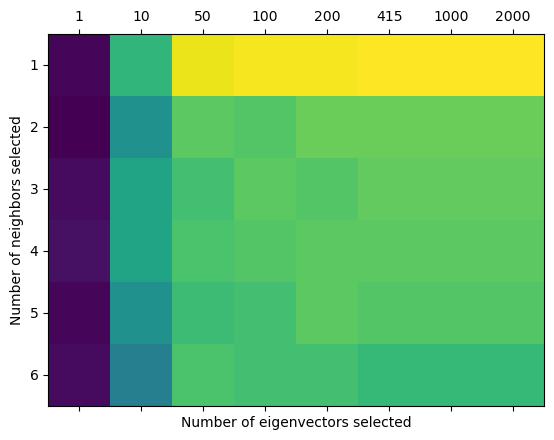
\includegraphics[width=8.0cm]{./Ressources/matrix_neighbors_eigenvectors.png}
%	\caption{Reconstruction error with different neighbors}
%	\label{fig:knn_num}
%\end{figure}

\begin{figure}[h]
	\centering
	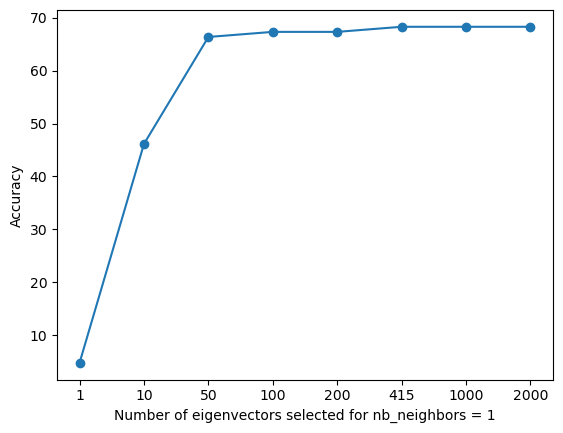
\includegraphics[width=8.0cm]{./Ressources/accuracy_1neighbors.png}
	\caption{Reconstruction error with different components}
	\label{fig:n_num}
\end{figure}
We calculated the accuracy at different values of neighbors and finally found that the accuracy at n\_neighbors=1 is significantly higher than other values.

Then, from the Figure~\ref{fig:n_num} we can see that the best results are obtained with n\_neighbors = 1 for the NN classifier and that the higher the number of components, the better the classification.

\begin{figure}[h]
	\centering
	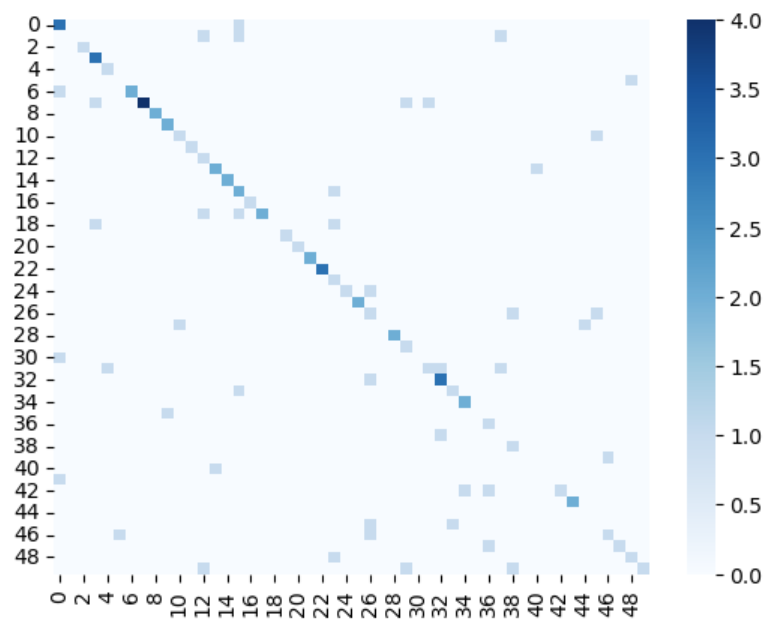
\includegraphics[width=8.0cm]{./Ressources/Q1_cm.png}
	\caption{Confusion Matrix}
	\label{fig:Q1_cm}
\end{figure}
And the Figure~\ref{fig:Q1_cm} shows that the classification effect of the model is not very good, because there are some dark points located outside the diagonal (that is, prediction errors).




